\documentclass[11pt]{article}
\usepackage[margin=1in]{geometry}
\usepackage[numbers,sort&compress,round]{natbib}
\usepackage[utf8]{inputenc}
\usepackage[T1]{fontenc}
\usepackage{lmodern}
\usepackage{hyperref,url,booktabs,amsmath,amssymb,graphicx,float}
\graphicspath{{figures/}}
\title{\textbf{Behavioural repertoires tile the identifiable parameter subspaces of whole-organism nervous-system models}}
\author{Chenxi He \\ Cavendish Laboratory, University of Cambridge \\ \texttt{ch2067@cam.ac.uk}}
\date{}

\begin{document}
\maketitle

\begin{abstract}
\noindent
Whole-organism biophysical simulators reproduce animal behaviour from hundreds to thousands of internal parameters, yet how many of those parameters behaviour actually constrains is unknown. Here we measure the behavioural-equivalence manifold, the set of parameter configurations that yield indistinguishable behaviour, across simulators spanning three phyla. We find that behaviour constrains a low-dimensional stiff subspace and leaves the remaining directions free, and we characterise that subspace in three ways. Its identity: in the nematode it is the neural substrate of the animal's four-dimensional postural repertoire, and two independently built models generate behaviour that occupies the measured eigenworm space. Its dependence on behaviour: distinct behaviours constrain complementary rather than overlapping subspaces, so that the identifiable dimension is the union over the behavioural repertoire and grows as behaviours are added, which we demonstrate in nematode, fly-larva and rodent models. Its generality: the same organisation, with network connectivity and slow membrane properties stiff and fast voltage-gated inward currents sloppy, recurs in every system examined and in four independent biological datasets that use none of our simulators. In these models, behaviour therefore constrains a low-dimensional subspace whose extent is set by behavioural richness, leaving a residual set of directions that no behaviour in the repertoire constrains.
\end{abstract}

% ============ INTRODUCTION ============
\section*{Introduction}
A central premise of mechanistic whole-organism simulators is that fitting them to behaviour recovers the biophysics that produces it. Decades of work on conductance-based models, however---from the stomatogastric ganglion \citep{prinz2004similar,marder2006variability} to the broader theory of sloppy models \citep{gutenkunst2007universally,transtrum2015perspective}---establish that many parameter sets produce indistinguishable dynamics: the map from parameters to behaviour is many-to-one \citep{goldman2001global,taylor2009how,marder2011variability,edelman2001degeneracy,alonso2019visualization}. Whether, and how strongly, this degeneracy holds at the scale of a \emph{whole-organism} nervous system---thousands of synaptic, junctional and channel parameters driving a behaving body---has not been measured. The consequences are direct: if behaviour constrains only a low-dimensional subspace, then behaviour-based calibration can recover that subspace but not the remainder, and the parameters it leaves unconstrained are candidates for the directions along which biology can vary without behavioural consequence.

Here we measure the behavioural-equivalence manifold of four published whole-organism motor simulators (BAAIWorm \citep{wang2025baaiworm}, modWorm \citep{shlizerman2025modworm}, flybody \citep{vaxenburg2025flybody}, and NeuroMechFly~v2 / FlyGym \citep{wangchen2024neuromechfly,lobatorios2022neuromechfly}), which are built on physics engines for musculoskeletal control \citep{todorov2012mujoco,delp2007opensim}. To test generality, we extend the same measurement across three phyla by adding a fly-larva model, a mammalian model, a connectome-constrained \emph{Drosophila} visual circuit and the canonical crustacean pyloric population. We do not attempt to recover the true parameters; rather, we measure the manifold of behaviourally equivalent ones, identify the constrained (stiff) subspace, and ask whether its low-dimensional geometry recurs across systems and in biology. The contribution is a measurement, together with convergent observations from biological data that use none of these models.

The components required to do this at scale are now available. Connectome-constrained whole-organism simulators rest on increasingly complete wiring diagrams \citep{white1986structure,varshney2011structural,cook2019connectome,witvliet2021connectomes,yan2017network,scheffer2020connectome,dorkenwald2024flywire,azevedo2024connectomic} on community simulation frameworks \citep{szigeti2014openworm,sarma2018openworm,gleeson2018c302,hines1997neuron}, and on the whole-brain neural recordings they aim to reproduce \citep{kato2015global,nguyen2016whole,randi2023multimodal}; high-throughput tracking reduces behaviour to low-dimensional kinematic descriptors \citep{stephens2008dimensionality,stephens2011emergence,brown2013dictionary,yemini2013openworm,javer2018open,pereira2022sleap,karashchuk2021anipose,pereira2020quantifying}; and parameter inference is increasingly amortised by simulation-based methods \citep{cranmer2020frontier,goncalves2020training,tejero2020sbi,papamakarios2017maf,durkan2019nsf} or performed by black-box optimisers \citep{spall1992multivariate,hansen2001completely,hansen2016cma,spall2003introduction}; behaviour-based parameter generation for whole-organism simulators has recently been demonstrated from tracking video alone \citep{he2026pgob}. What none of these components settles is \emph{how much} of a whole-organism parameter set behaviour actually determines---the classical identifiability question \citep{villaverde2014reverse,saltelli2008global} that sloppy-model theory answers for small systems \citep{gutenkunst2007universally,transtrum2015perspective,sethna2010sloppy,transtrum2010sloppy} and that pyloric degeneracy answers for a single circuit \citep{prinz2004similar,marder2006variability}. Quantifying it at whole-organism scale is a prerequisite for behaviourally grounded digital organisms \citep{karr2012whole,zador2023catalyzing,urai2022largescale,bargmann2013connectome}.

% ============ RESULTS ============
\section*{Results}

\subsection*{Behaviour converges while parameters remain dispersed}
We first asked whether the manifold has positive dimension. Repeating optimisation from independent starting points against a single fixed behavioural target, the behavioural loss converged while the recovered parameter vectors remained dispersed. On the $126$-dimensional FlyGym controller, $29$ of $30$ runs reach the behavioural target while the solution cloud occupies an effective $21.7$ of $126$ dimensions; on the full coupled real modWorm model (OpenWorm connectome, $279$ neurons), the behavioural curvature concentrates on $2$ of $7$ mechanism directions (Hessian analysis below), leaving the remainder unconstrained. Behavioural convergence with persistent parameter dispersion is direct evidence that the equivalence manifold has positive dimension (Fig.~\ref{fig:manifold}a).

\subsection*{The behavioural-equivalence manifold is low-dimensional}
We next quantified the dimensionality directly from the behavioural-loss Hessian at the optimum. On the $767$-parameter flybody policy, a Lanczos spectrum yielded $6$ stiff directions at $90\%$ and $11$ at $99\%$ of the spectral mass, with $28$ of $40$ sampled directions flat to $|\lambda|\sim10^{-11}$. On the full coupled real modWorm model, the per-mechanism behavioural Hessian had effective dimension $2$ of $7$ (synaptic, gap-junction and synaptic rise-time directions stiff; capacitance and gain sloppy). On the $48$-dimensional FlyGym walking controller, the behavioural Hessian had effective dimension $3$ ($90\%$) / $6$ ($99\%$) of $48$ and spanned $19.5$ orders of magnitude. On BAAIWorm, the Gauss--Newton curvature over $20$ named mechanisms had effective dimension $2$ ($90\%$) / $3$ ($99\%$) of $20$. Across parameter counts of $7$, $20$, $48$ and $767$, behaviour is set by a low-dimensional stiff subspace embedded in a high-dimensional flat manifold (Fig.~\ref{fig:manifold}b).

\begin{figure}[H]
\centering
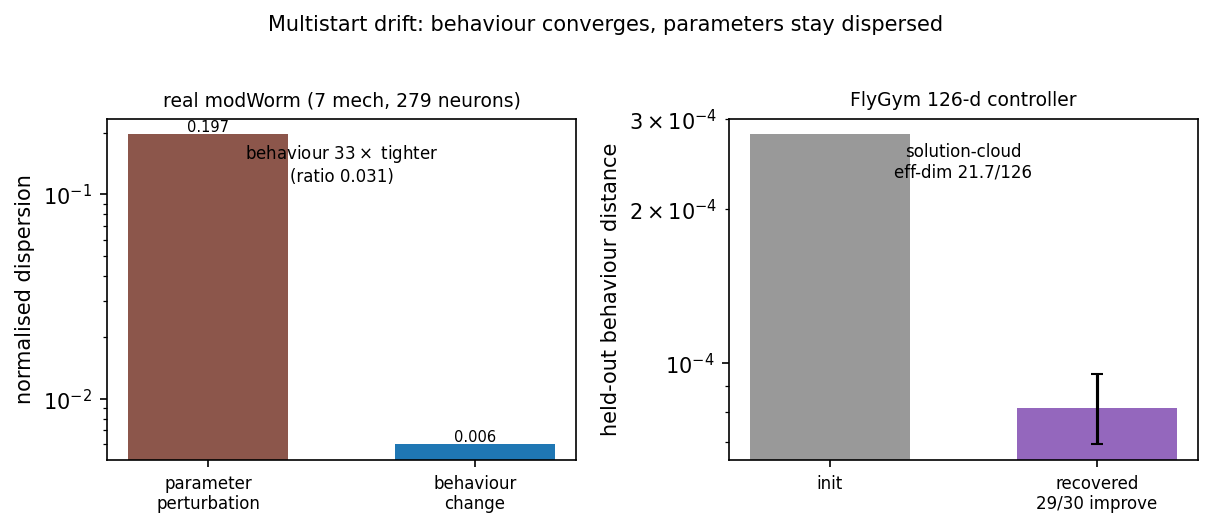
\includegraphics[width=0.48\textwidth]{Fig_multistart_three_sim.png}\hfill
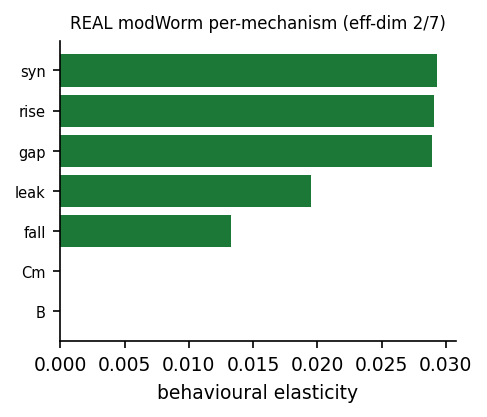
\includegraphics[width=0.48\textwidth]{fig_p2_modworm_real_b1.png}
\caption{\textbf{The behavioural-equivalence manifold, measured.} \textbf{a}, Multistart drift: independent optimisations converge in behaviour while the recovered parameters remain dispersed (FlyGym $29/30$ behavioural success, solution-cloud effective dimension $21.7/126$; real modWorm behaviour approximately $30\times$ less variable than its parameters), indicating a positive-dimensional manifold. \textbf{b}, Gauss--Newton behavioural curvature per biophysical mechanism on the full coupled real modWorm model (OpenWorm connectome, $279$ neurons). The synaptic and gap-junction conductances and the synaptic rise time carry the curvature, whereas the membrane capacitance and the sigmoid gain are behaviourally flat, giving an effective dimension of $2$ of $7$: a small number of stiff directions and many sloppy ones.}
\label{fig:manifold}
\end{figure}

\subsection*{The manifold is the neural control of eigenworm posture}
The nematode behavioural manifold is not an abstract low-dimensional set but the parameter-space image of the animal's known approximately four-dimensional postural repertoire. Real \emph{C.~elegans} posture from the OpenWorm Movement Database occupied an effective $3.79$--$4.14$ dimensions, with four eigenworms capturing $94$--$96\%$ of postural variance, reproducing the classical eigenworm decomposition \citep{stephens2008dimensionality}. Two independently constructed worm models generated behaviour occupying this same empirical eigenworm space: the modWorm posture subspace aligned with the real eigenworm basis at $\cos\,0.77$ and BAAIWorm at $\cos\,0.68$--$0.69$ ($67$--$72\%$ of variance). These alignments substantially exceeded those of random four-dimensional subspaces (modWorm $p{=}0.001$, BAAIWorm $p{=}0.04$ even within a conservative ten-dimensional posture ambient; $p{<}10^{-4}$ in the full space; Supplementary~\S6.1), and within each model it was the stiff mechanisms, not the sloppy ones, that displaced the eigenworm trajectory. In the systems examined here the effective rank of behavioural sensitivity tracks the intrinsic dimensionality of the postural repertoire, rather than the number of observables recorded: re-measuring with $7{,}200$--$14{,}400$ posture observables in place of six summary kinematics left the effective dimension at $2$--$3$ of $7$ (Supplementary~\S6.2). We note that this is an empirical property of these models and behavioural losses, not a general bound: a low-dimensional attractor can in principle constrain many parameter combinations through transients, multiple initial conditions or nonlinear temporal structure, and the intrinsic dimensionality of the behaviour need not equal the rank of the parameter-to-trajectory Jacobian. The low-dimensional behavioural-equivalence manifold is thus the neural control of the animal's low-dimensional posture (Fig.~\ref{fig:tiling}a).

\subsection*{Distinct behaviours constrain complementary subspaces}
A low-dimensional behaviour raises the question of how a whole nervous system could be identified at all. The resolution is that distinct behaviours do not constrain the \emph{same} few directions but complementary ones. In BAAIWorm, perturbing the chemosensory parameters altered behaviour $7.15\times$ more during chemotaxis (food-directed; sensitivity $0.872$) than during plain locomotion in a weak gradient ($0.122$), whereas perturbing the motor parameters showed the opposite contrast ($0.109$ versus $0.357$): the axis a behaviour renders stiff is the axis its function requires, and chemotaxis and locomotion render \emph{different} axes stiff. This is consistent with the anatomical separation of the chemosensory navigation circuit from the ventral-cord locomotor circuit \citep{gray2005circuit,bargmann2012beyond}, and with models in which distinct premotor and motor elements generate the locomotor rhythm \citep{wen2012proprioceptive,fouad2018distributed,gao2018excitatory,boyle2012gait,izquierdo2018connecting,rakowski2017optimal}. The identifiable subspace is therefore not the few directions of any single behaviour but the union over the behavioural repertoire. Within a single worm model this union increased as behaviours were added: four distinct locomotor presets each constrained $2$--$4$ of $7$ mechanism directions with only partial overlap (mean pairwise stiff-subspace $\cos\,0.54$); their behaviour-specific stiff directions spanned an effective $2.98$ of $4$ dimensions, each behaviour contributing on average a $0.54$ component orthogonal to the others. Because a union necessarily grows whenever subspaces are not identical, we tested this against two explicit nulls. Randomly oriented directions in the same space would span $3.50$ dimensions ($95\%$ interval $3.00$--$3.88$) with mean pairwise $\cos\,0.31$, whereas a single shared direction would span $1$ with $\cos\,1$. The observed geometry lies between the two and is significantly more aligned than random ($p{=}0.020$ for the span, $p{=}0.016$ for the pairwise cosine, $20{,}000$ draws): the behaviours share substantial structure while each still contributes a distinct component, so the growth of the union is neither redundancy nor the trivial consequence of non-identical subspaces (Supplementary~\S6.4). Their union reached $5$; across twelve behaviours it saturated at $4$ of $7$, leaving a residual $2$--$3$ directions that no behaviour constrains, an irreducible degenerate core. The stiff and sloppy directions are distributed parameter combinations rather than single parameters (stiff-subspace participation $3.42$, sloppy $4.68$ of $7$), so this core is a genuine biological neutral space and not an unused parameter (Fig.~\ref{fig:tiling}b,c).

\subsection*{The same geometry recurs across three phyla}
This low-dimensional, complementarily tiled organisation is not specific to the nematode. We measured it also in a fly larva (larvaworld) and a mammal (Virtual Rodent \citep{merel2019deep,aldarondo2024virtual}, 	exttt{dm\_control} \citep{tunyasuvunakool2020dmcontrol,tassa2018deepmind}), and in each case the identifiable dimension increased as distinct behaviours were added rather than being fixed by any one behaviour. In the larva, four genuinely distinct sensory behaviours (free exploration, chemotaxis, anemotaxis and feeding) each engage a different module---olfactory, wind-sensory and feeding---so that their union ($8$ of $10$) was approximately double the single-behaviour dimension ($3$--$5$). In the rodent, a six-behaviour repertoire drove a still-increasing identifiability curve ($3.7\to12$ of $38$ actuators). The absolute counts are not comparable across species, as the three models are parameterised differently and the rodent is driven open-loop, but the structure is invariant: a low-dimensional stiff subspace per behaviour, complementary across behaviours, with an identifiable dimension set by behavioural richness. The crustacean pyloric population and a \emph{Drosophila} visual circuit (below) extend the same stiff/sloppy geometry to a fourth and fifth system (Fig.~\ref{fig:tiling}d).

\begin{figure}[H]
\centering
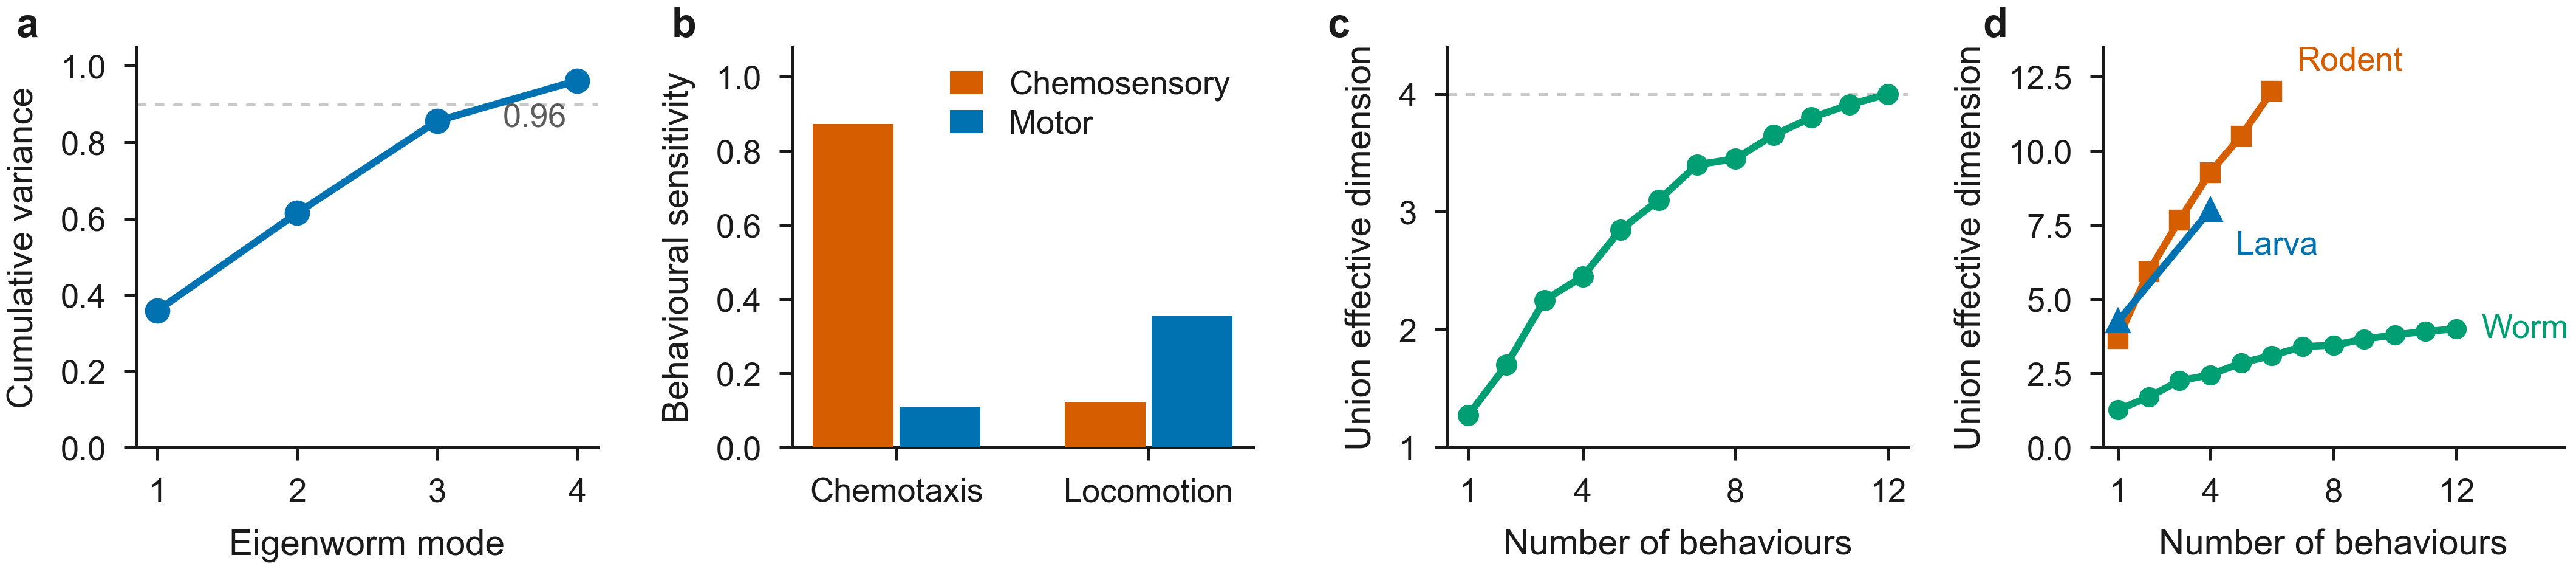
\includegraphics[width=0.98\textwidth]{fig_p2_tiling_crossspecies.png}
\caption{\textbf{The identifiable subspace is the eigenworm space, tiled complementarily by behaviour, across phyla.} \textbf{a}, Cumulative postural variance of real \emph{C.~elegans} posture (OpenWorm Movement Database, $n{=}8432$ frames) across eigenworm modes; four modes capture $0.96$ of the variance (dashed line, $0.90$). Two independently constructed worm models align with this empirical basis at $\cos\,0.77$ (modWorm) and $\cos\,0.68$ (BAAIWorm). \textbf{b}, Behavioural sensitivity to perturbation of the chemosensory (vermillion) and motor (blue) parameter classes, during food-directed chemotaxis and during plain locomotion in a weak gradient. Chemosensory parameters are stiff during chemotaxis but sloppy during locomotion (a $7.15\times$ context shift) and motor parameters show the reverse contrast, so distinct behaviours constrain distinct axes. \textbf{c}, Union effective dimension of the identifiable subspace as behaviours are added (real modWorm, twelve behaviours), saturating at $4$ of $7$ mechanism directions (dashed line) and leaving a residual degenerate core. \textbf{d}, The same increase with repertoire size in three phyla: nematode (green, $7$ mechanisms), fly larva (blue, $10$ parameters) and rodent (vermillion, $38$ actuators). Absolute counts are not comparable across species because the models are parameterised differently; the structure is invariant.}
\label{fig:tiling}
\end{figure}

\subsection*{Two independent probes agree on the identifiable axes}
Computed on the full coupled real modWorm model within a single shared prior region (per-mechanism log-multipliers, prior scale $0.15$), the two geometric probes concurred on which axes are identifiable: per-mechanism Hessian stiffness and negative manifold drift were rank-correlated at Spearman $\rho{=}0.96$ ($p{=}5\times10^{-4}$, $7$ mechanisms). A third probe served as a calibration control rather than a parallel identifiability ranking: an amortised neural posterior (NPE/MAF, \texttt{sbi}) trained in the same region on $N{=}300$ real simulations was well-calibrated on all $7$ mechanisms (per-axis simulation-based calibration passes $7/7$; Kolmogorov--Smirnov $p>0.05$). This confirms that the inference is sound but, because a calibrated posterior calibrates every axis, does not by itself yield a per-axis stiff/sloppy ordering. We therefore read the manifold's stiff/sloppy geometry from the two probes that agree, using simulation-based calibration as a control on the inference.

\subsection*{Stiff and sloppy directions are biophysically interpretable}
Decomposing the BAAIWorm behavioural curvature over $20$ named mechanisms (Supplementary~\S5.2) gives a positive semi-definite Gauss--Newton spectrum ($43.2$, $5.84$, $0.88$, $0.47$, remainder at the finite-difference floor) with effective dimension $2$ ($90\%$) / $3$ ($99\%$) of $20$, and resolves the partition by mechanism: the stiffest axes are the passive leak, the gap-junction and synaptic weights, the motor output and several potassium conductances, whereas the fast voltage-gated calcium channels EGL-19 and UNC-2 and the calcium-activated potassium channels SLO-1/SLO-2 are the sloppiest. Behaviour is thus determined by how cells are connected and by their passive and slow properties, and is largely insensitive to the fast voltage-gated calcium conductances, consistent with the known compensation and variability of these currents in small circuits \citep{marder2006variability}. A complementary probe over the full $3076$-weight connectome found the connection weights collectively stiff (Supplementary~\S5.3), locating the degeneracy in the single-cell biophysics rather than in the connectivity. This partition is not an artefact of one model: probed identically, two independently constructed worm simulators---modWorm (coupled-ODE, $7$ mechanisms) and BAAIWorm (NEURON, $20$ named channels)---agree that the network-connectivity axes are stiff (stiff fraction $0.83$ / $0.87$) while the single-cell biophysical axes are sloppy ($0.08$ / $0.16$), indicating that ``connectivity stiff, single-cell sloppy'' is reproducible across independent implementations of the same organism rather than an artefact of one model.

\begin{figure}[H]
\centering
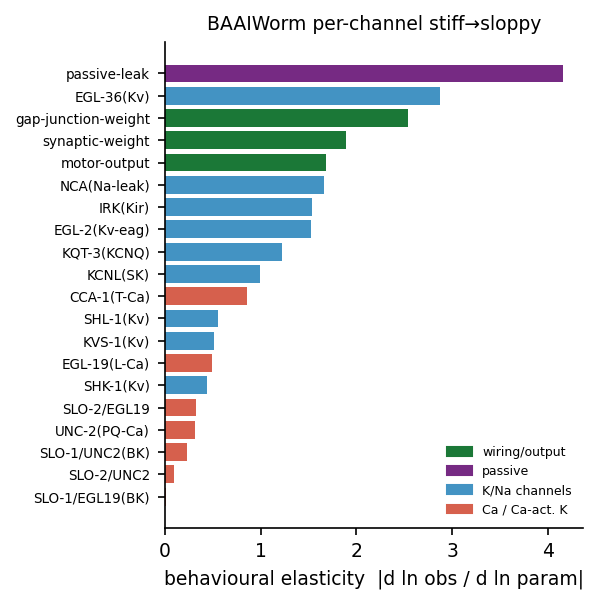
\includegraphics[width=0.46\textwidth]{fig_p2_b1_perchannel.png}\hfill
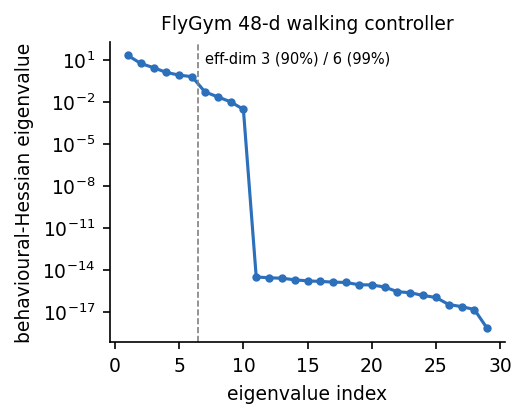
\includegraphics[width=0.46\textwidth]{fig_p2_flygym_hessian48.png}
\caption{\textbf{Stiff/sloppy structure at named-channel and higher-dimensional scale.} Left: BAAIWorm per-channel behavioural elasticity over $20$ named mechanisms, ordered stiff (top) to sloppy (bottom); the connectivity (gap-junction, synaptic and motor) and passive-leak axes are stiff, and the fast voltage-gated calcium channels EGL-19/UNC-2 and the calcium-activated potassium channels SLO-1/SLO-2 are sloppy. Right: behavioural-Hessian eigenspectrum of the $48$-dimensional FlyGym walking controller, effective dimension $3$--$6$ of $48$.}
\label{fig:perchannel}
\end{figure}

\subsection*{Convergent observations in independent biological data}
Four independent datasets, none of which involves our forward models, exhibit low-dimensional or graded stiff/sloppy structure of the same kind (Fig.~\ref{fig:external}). These are convergent observations rather than a direct validation: they compare different levels of description---model-parameter curvature, neuronal phenotype variability, protein-sequence conservation and cross-individual behavioural variation---and so establish qualitative consistency rather than a correspondence between individual eigenvectors.
\emph{(1) Pyloric degeneracy.} Applying our Hessian probe to the Prinz--Marder population of conductance-based models that produce the same triphasic pyloric rhythm \citep{prinz2004similar} (rhythm-validity gated; valid rate $0.56\%$) yielded a $31$-parameter eigenspectrum spanning approximately ten orders of magnitude with effective dimension $2.13/31$---only $2$--$6$ stiff directions, with stiffness on the leak and inhibitory-synapse conductances and sloppiness on the fast sodium conductances, the currents known to be compensated in this circuit. This canonical degeneracy dataset exhibits the same low-dimensional stiff/sloppy partition as the simulators.
\emph{(2) Neuronal property variability.} Across $n{=}1914$ Allen cortical neurons, electrophysiological properties span a stiff/sloppy gradient (coefficient of variation $0.08$--$1.85$: resting potential stiff, adaptation and firing rate sloppy) on a property-space manifold of participation dimension $4.78/11$.
\emph{(3) Gene conservation.} Across $40$ \emph{C.~elegans} ion-channel and synaptic genes, ortholog identity across \emph{Caenorhabditis} ranges from $77.9$ to $99.9\%$; the gap-junction gene \texttt{unc-9} is the single most conserved ($99.9\%$), paralleling the stiffness of the gap-junction axis in (1).
\emph{(4) Behavioural variation.} Across $n{=}61$ isogenic N2 worms ($683$ Tierpsy features), cross-individual behaviour occupies a participation dimension of $9.75$; genetically identical animals vary on an approximately ten-dimensional behavioural manifold, the empirical counterpart of the parameter manifold.
The directions that biology conserves and those it permits to vary are ordered consistently with the models' identifiable and degenerate axes, at the level of low-dimensionality and qualitative direction.

\begin{figure}[H]
\centering
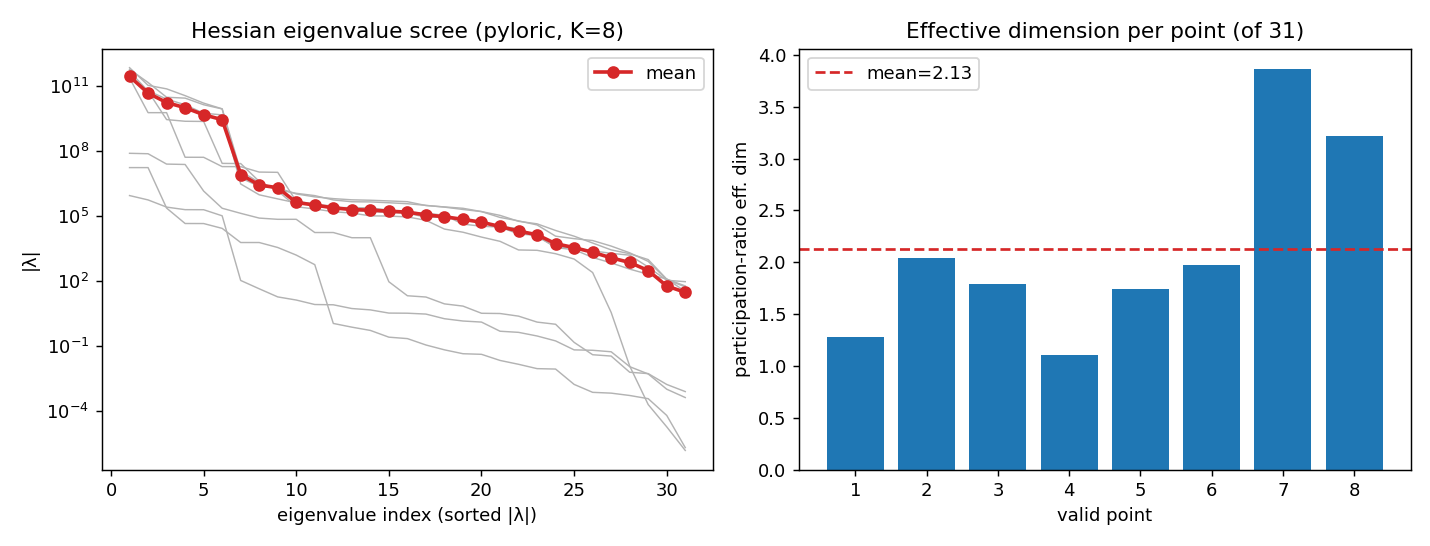
\includegraphics[width=0.48\textwidth]{e1b_hessian.png}\hfill
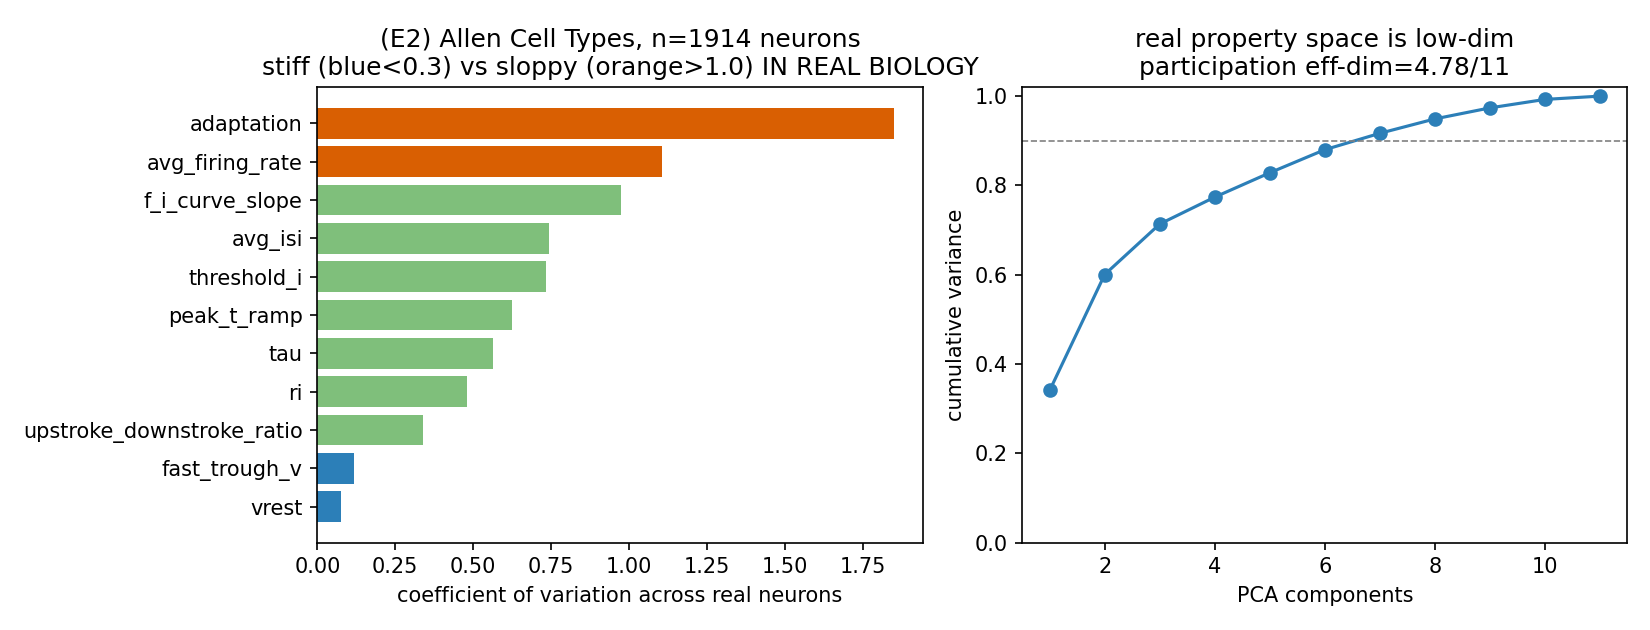
\includegraphics[width=0.48\textwidth]{Fig_E2_allen.png}\\[2pt]
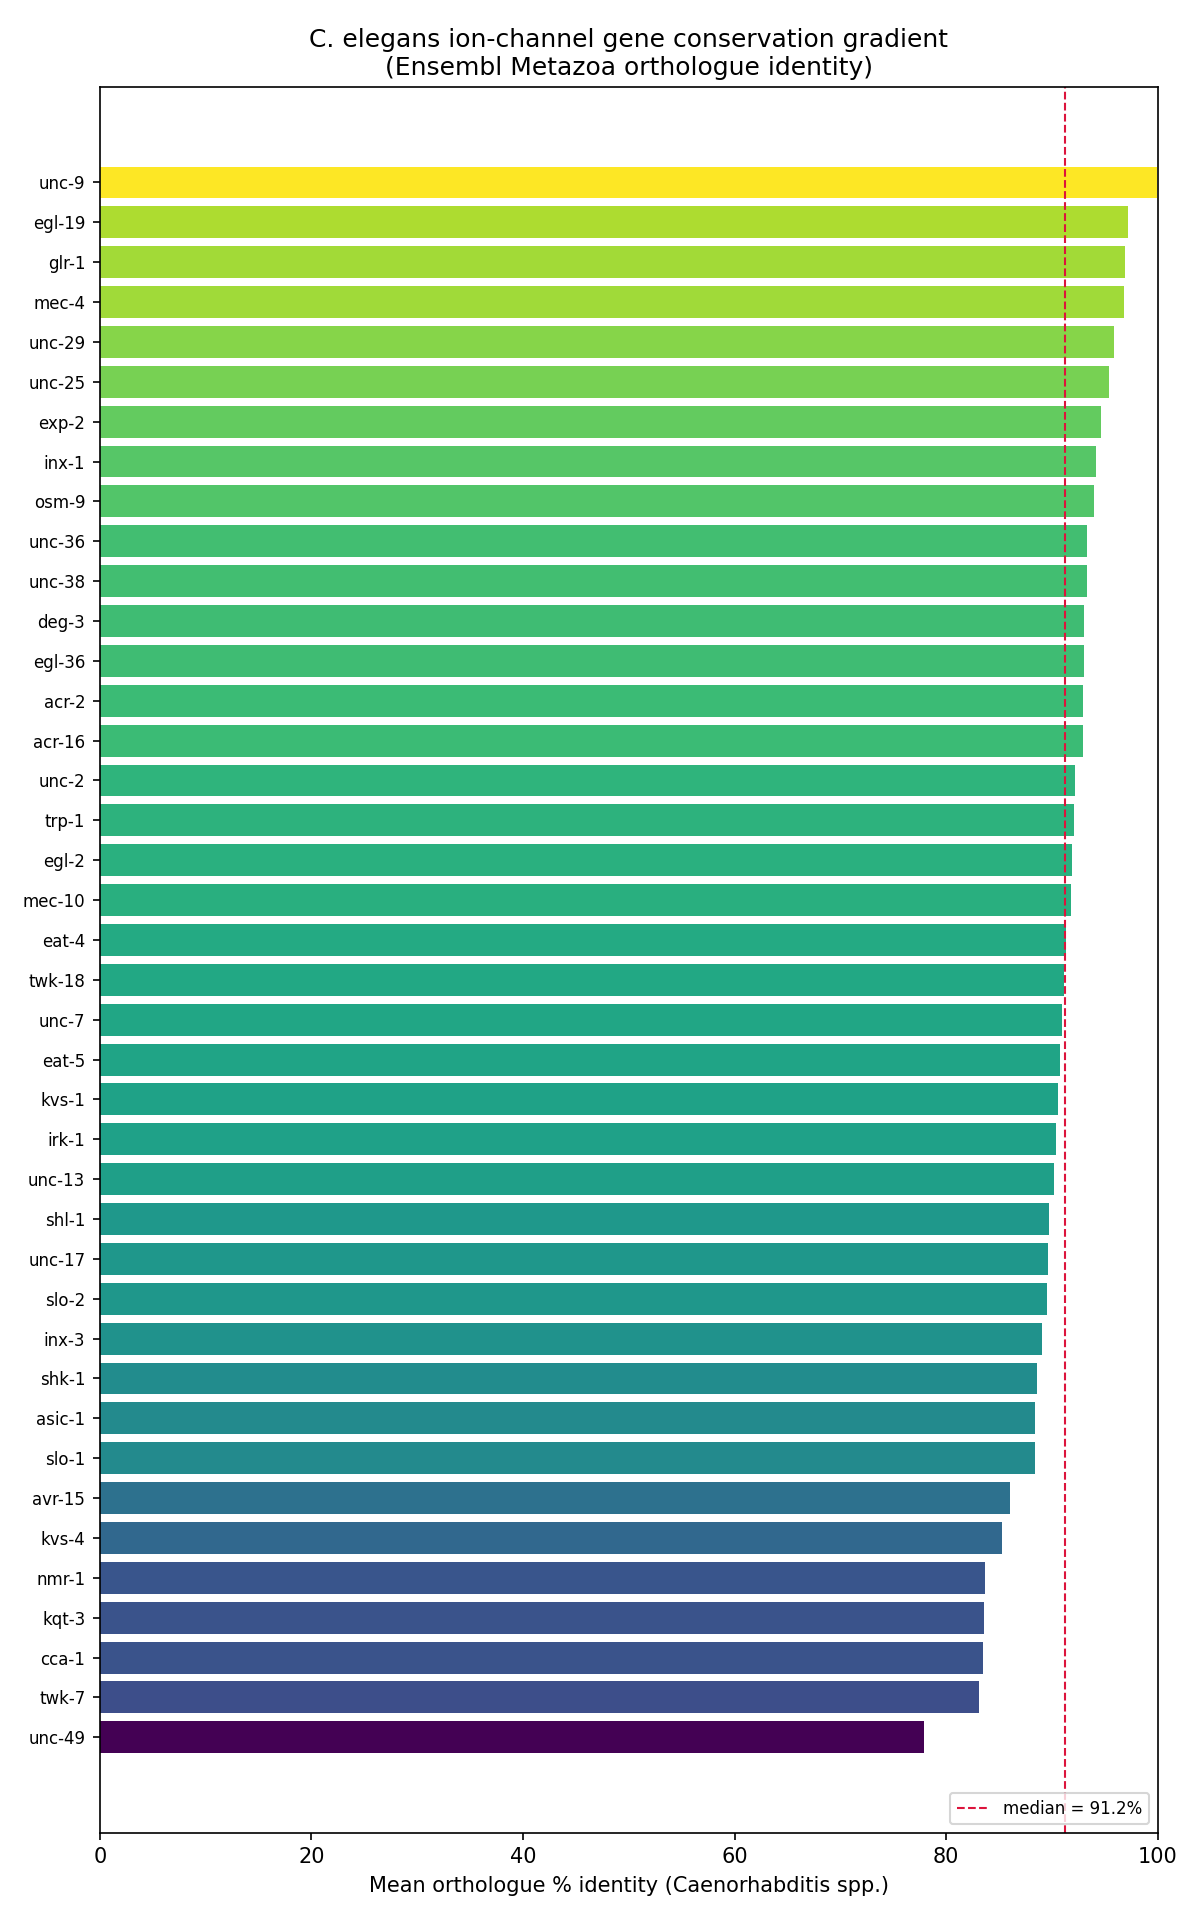
\includegraphics[width=0.48\textwidth]{Fig_E4_conservation.png}\hfill
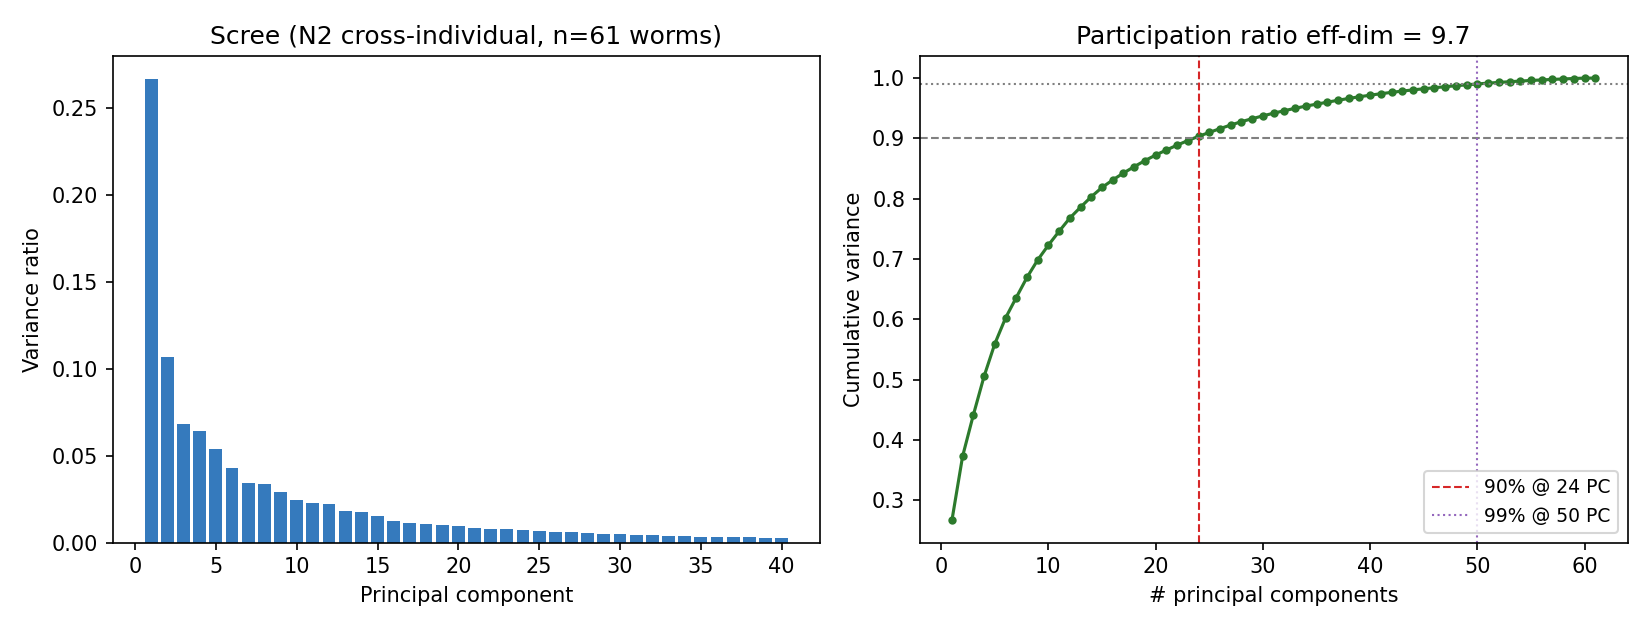
\includegraphics[width=0.48\textwidth]{Fig_E5_n2_manifold.png}
\caption{\textbf{The same low-dimensional stiff/sloppy geometry in four biological datasets that do not use our simulators.} Top-left: Prinz--Marder pyloric model population, rhythm-gated, $31$-parameter Hessian eigenspectrum (effective dimension $2.13/31$; stiff $=$ leak and inhibitory synapses, sloppy $=$ fast sodium). Top-right: Allen cortical-neuron property variability ($n{=}1914$; stiff/sloppy coefficient-of-variation gradient, participation dimension $4.78/11$). Bottom-left: \emph{C.~elegans} ion-channel-gene conservation across \emph{Caenorhabditis} ($n{=}40$ genes; \texttt{unc-9} gap junction most conserved). Bottom-right: isogenic-N2 behavioural manifold (OWMD, $n{=}61$ worms, $683$ Tierpsy features; participation dimension $9.75$).}
\label{fig:external}
\end{figure}

% ============ DISCUSSION ============
\section*{Discussion}
Whole-organism nervous-system models are extensively non-identifiable from behaviour, but the non-identifiability is structured, and the structure has a simple organising principle: what behaviour can identify is set by how rich the behaviour is. Any single behaviour is low-dimensional---in the nematode, the approximately four-dimensional eigenworm space---and constrains only a few stiff parameter combinations; but distinct behaviours constrain complementary combinations, those that their particular function requires (chemotaxis the chemosensory axes, locomotion the motor axes), so that the identifiable subspace is the union over the behavioural repertoire and increases with the repertoire. This recasts degeneracy as a measurable resource rather than a fixed limit: a connectome-constrained simulator is identifiable up to the diversity of behaviours one is willing to elicit and measure, and the directions that remain after every behaviour has been used---the residual degenerate core---are the directions that no behaviour in the repertoire constrains, and therefore candidate neutral directions. The result lifts the sloppy-models picture \citep{gutenkunst2007universally,transtrum2015perspective,sethna2010sloppy} and pyloric degeneracy \citep{prinz2004similar,marder2011variability} from single circuits to behaving whole organisms, and it explains why behaviour-based calibration recovers a working parameter set without recovering unique biophysical values: it recovers the stiff union, not the core. The unconstrained directions are not merely numerical: the independent datasets indicate that they tend also to be the more variable and less conserved directions in biology (cortical-property variability; cross-\emph{Caenorhabditis} gene conservation), consistent with the biophysical diversity documented within identified cell types \citep{gjorgjieva2016computational,oconnor2024neural}, so that the manifold is a map of which mechanisms behaviour can and cannot identify. A contrasting case bounds the scope of the low-dimensional result. Applying the same probe to a connectome-constrained \emph{Drosophila} visual model (Supplementary~\S5.7) yields a much higher effective dimension ($43$ of $65$ cell types) over a far narrower spectrum ($2.9$ orders of magnitude, against $19.5$ for the FlyGym walking controller), while the stiff axes remain the functionally load-bearing ones, here the T4/T5 motion-detector pathway. Low dimensionality is therefore a property of the whole-body motor systems we measured rather than of connectome-constrained models in general. We can exclude one trivial explanation for the contrast: it is not driven by the number of observables, since the worm analysis used $14{,}400$ posture observables against $64$ readouts here and still gave an effective dimension of $2$--$3$. Two differences nevertheless remain uncontrolled---the visual model is parameterised per cell type rather than per biophysical mechanism class, and a drifting-grating response is a different kind of output from locomotion---so we treat the relation between identifiable rank and task complexity as a testable prediction rather than an established invariant. Testing it properly requires plotting identifiable rank against an independently defined measure of output complexity across systems, with parameterisation granularity held fixed.

\paragraph{Limitations.} The per-channel decomposition (Supplementary~\S5.2) reaches named single conductances but still scales each conductance type uniformly across cells rather than cell by cell; the mapping from parameter axes to biophysical classes is biophysically informed rather than learned; and the alignment between simulator stiff axes and the external biological datasets (1)--(4) is established at the level of low-dimensionality and qualitative direction rather than per-eigenvector correspondence. The behaviour-to-neural prediction that would close the loop is confirmed only qualitatively---behaviour-recovered parameters reproduce the gross statistics (dimensionality, correlation scale) of the unobserved neural state, but in the modality of membrane voltage compared against immobilised calcium imaging (Supplementary~\S5.4), not as a per-neuron match. An external check of the stiff/sloppy ordering against real mutant phenotypes remains data-limited (Supplementary~\S5.6).

% ============ METHODS ============
\section*{Methods}
\textbf{Manifold drift.} For each simulator, $N$ optimisations (separable CMA-ES or SPSA) from independent starts are fitted to one fixed behavioural target; we report behavioural recovery, the normalised per-dimension dispersion of the $N$ recovered parameter vectors, and the PCA participation dimension of the solution cloud. \textbf{Behavioural curvature.} All curvature reported here is the Gauss--Newton form $H=J^\top W J$, built from the finite-difference observable Jacobian $J_{ik}=\partial\,\mathrm{obs}_i/\partial\theta_k$ and a diagonal positive semi-definite whitening matrix $W$ of inverse per-observable scales. $H$ is therefore positive semi-definite by construction and equals the Fisher information of the parameters given the behavioural observables, so its eigenvalues are non-negative and its effective dimension is the local practical-identifiability rank in the standard sense \citep{villaverde2014reverse,gutenkunst2007universally}. Eigenvalues are obtained by direct eigendecomposition (low dimension) or Lanczos iteration (high dimension). The effective dimension at level $q$ is the smallest $k$ such that $\sum_{i\le k}\lambda_i \ge q\sum_i \lambda_i$ with eigenvalues sorted in decreasing order; we report $q=0.90$ and $q=0.99$, together with the threshold-free participation ratio $(\sum_i\lambda_i)^2/\sum_i\lambda_i^2$ (Supplementary~\S6.9). A direction counts as flat when $\lambda$ falls to the finite-difference floor; residual eigenvalues of magnitude below that floor, of either sign, are numerical noise and are treated as zero. We adopt it as the primary cross-simulator metric because it is robust to the choice of observable and parameterisation, unlike a raw perturbation-sensitivity ratio, and because the manifold-drift probe provides an independent, optimisation-based cross-check that agrees with it ($\rho{=}0.96$). \textbf{Eigenworm identity.} Real \emph{C.~elegans} skeletons (OWMD N2) and model body postures are reduced to tangent-angle eigenmodes by PCA; we report the posture effective dimension, the top-four cumulative variance, and the principal-angle cosine between model and real eigenworm subspaces, with significance assessed against random subspaces of matched dimension. \textbf{Complementary tiling and saturation.} Per-behaviour stiff subspaces are taken as the leading Hessian eigenvectors under each behavioural target; we report pairwise stiff-subspace cosines, the union effective dimension over a behaviour set, and the saturation curve of union dimension against the number of behaviours. Context dependence (BAAIWorm) is the ratio of a parameter class's behavioural sensitivity between two behaviours (chemotaxis versus weak-gradient locomotion). The same union/saturation construction is applied across species (fly larva, larvaworld; rodent, Virtual Rodent / dm\_control). \textbf{Calibration.} Per-dimension rank-based simulation-based calibration \citep{talts2018validating,hermans2022sbc} of an amortised neural posterior \citep{papamakarios2016mdn,deistler2022truncated}; a dimension passes when the per-axis Kolmogorov--Smirnov test is non-significant at $\alpha{=}0.05$. \textbf{External datasets.} The Prinz--Marder pyloric model population re-gated to the triphasic rhythm and probed with the identical Hessian-eigenspectrum method; Allen Cell Types electrophysiology; WormBase ParaSite / Ensembl Metazoa ortholog identities; and OpenWorm Movement Database isogenic-N2 Tierpsy features. All external data are public, and no simulator is used in datasets (1)--(4). Full specifications, cohort sizes and reproduction commands are given in the Supplementary Information.

% ============ DECLARATIONS ============
\section*{Data availability}
All datasets analysed in this study are publicly available. The external biological references are: the Prinz--Marder conductance-based model population of the stomatogastric ganglion \citep{prinz2004similar}; the Allen Cell Types electrophysiology database (\url{https://celltypes.brain-map.org}); ortholog identities from WormBase ParaSite and Ensembl Metazoa (\url{https://parasite.wormbase.org}); and the OpenWorm Movement Database (\url{http://movement.openworm.org}). The whole-organism simulators are the published releases of BAAIWorm \citep{wang2025baaiworm}, modWorm \citep{shlizerman2025modworm}, flybody \citep{vaxenburg2025flybody}, NeuroMechFly~v2 / FlyGym \citep{wangchen2024neuromechfly}, the connectome-constrained optic-lobe model of \citet{lappalainen2024connectome}, larvaworld, and the Virtual Rodent of the \texttt{dm\_control} suite. All quantities reported in the main text and Supplementary Information are provided as result files, one file per analysis as named in each Supplementary section, in the deposit at \url{https://github.com/ChenxiHeCam/behavioural-parameter-manifold}, archived at Zenodo (\url{https://doi.org/10.5281/zenodo.21594746}).

\section*{Code availability}
All analysis code, the per-experiment result files, and a container that reproduces every reported quantity and figure from those files are available at \url{https://github.com/ChenxiHeCam/behavioural-parameter-manifold} under an MIT licence, archived at Zenodo (\url{https://doi.org/10.5281/zenodo.21594746}). The reproduction entry point verifies each numerical claim against its source file and regenerates the figures.

\section*{Acknowledgements}
The author thanks the developers of the open-source whole-organism simulators and the curators of the public datasets used here, without which this study would not have been possible.

\section*{Author contributions}
C.H. conceived the study, designed and performed all analyses, and wrote the manuscript.

\section*{Competing interests}
The author declares no competing interests.

\bibliographystyle{unsrtnat}
\bibliography{references}
\end{document}
